\section{Introduction}

\subsection{Motivation}

Dans un monde où les consommateurs sont de plus en plus conscients des implications éthiques, environnementales et sanitaires de leurs achats, il est crucial de fournir des outils qui permettent de faire des choix éclairés. L'application Etiscan a été conçue pour répondre à ce besoin croissant. En scannant des produits, les utilisateurs peuvent obtenir des métadonnées détaillées et pertinentes sur ceux-ci. Ces informations permettent de savoir si un produit est local, équitable, biologique, ou répond à d'autres critères spécifiques que l'utilisateur juge importants. Etiscan offre une solution moderne et pratique pour aligner les choix de consommation avec les valeurs personnelles des individus.

\subsection{Concept}

L'application Etiscan se distingue par son approche innovante et personnalisée des métadonnées de produits. Contrairement à des applications existantes comme Yuka \cite{yuka}, qui se concentrent uniquement sur les métadonnées alimentaires, Etiscan vise à créer une plateforme versatile où les utilisateurs peuvent s'abonner aux types de métadonnées qui leur importent le plus. Des mainteneurs spécialisés testent les produits et certifient les informations, assurant ainsi la fiabilité des données fournies. Cette plateforme unique ambitionne de rassembler une large base d'utilisateurs en leur offrant une solution intégrée et complète pour suivre les produits en fonction de leurs préférences et convictions personnelles. En facilitant l'accès à des informations détaillées et certifiées, Etiscan se positionne comme un outil indispensable pour les consommateurs modernes et responsables.


\subsection{Vue d'ensemble des technologies}

Dans le développement de notre application mobile, nous avons adopté plusieurs technologies modernes pour garantir efficacité, performance et maintenabilité. Cette section présente une vue d'ensemble des technologies utilisées, organisées par front-end et back-end, ainsi que les outils de développement et de déploiement employés.

\begin{itemize}[noitemsep]
    \item \textbf{Framework principale :} Flutter
    \item \textbf{Versionnement et CI/CD :} GitHub, GitHub Actions
    \item \textbf{Authentification :} Firebase Authentication
    \item \textbf{Base de données :} Firebase Firestore
    \item \textbf{Scan de codes QR :} Librairie Google
    \item \textbf{Architecture :} Clean Architecture, Bloc
    \item \textbf{Automatisation de code :} JSON Serializable, Freezed
    \item \textbf{Localisation :} Localizations de base de Flutter
\end{itemize}

\subsection{Front-end}

Pour le développement de l'interface utilisateur, nous avons choisi Flutter comme framework principal. Flutter permet de créer des applications cross-platform, ce qui nous permet de cibler à la fois les utilisateurs Android et iOS avec une seule base de code. Voici quelques-unes des technologies et pratiques clés que nous avons utilisées pour le front-end :

\begin{itemize}[noitemsep]
    \item \textbf{Flutter :} Framework pour le développement d'interfaces utilisateur.
    \item \textbf{Bloc :} Utilisé pour la gestion de l'état, assurant une séparation claire des responsabilités et facilitant la testabilité.
    \item \textbf{Localizations :} Pour supporter plusieurs langues et offrir une expérience utilisateur adaptée à différents marchés.
    \item \textbf{Librairie Google pour QR code :} Intégrée pour offrir une fonctionnalité de scan rapide et précise.
\end{itemize}

\subsection{technologies de stockages}

Nous avons considéré différentes technologies pour stocker nos données avant de décider d'utiliser Firebase. Voici un aperçu de ces technologies de stockage utilisables sur Flutter, classées en deux catégories : SQL et NoSQL.

\subsubsection{SQL}

\begin{table}[h!]
    \centering
    \begin{tabular}{|c|c|c|}
    \hline
    \textbf{Technologie} & \textbf{Principales Fonctionnalités} & \textbf{Différences Notables} \\
    \hline
    SQFLite & Stockage SQL local fiable, contrôle fin des requêtes & Nécessite des connaissances en SQL \\
    \hline
    Drift & local, ORM avec sécurité des types, intégration réactive & Abstrait la complexité de SQLite \\
    \hline
    \end{tabular}
    \caption{Technologies SQL pour Flutter}
\end{table}

\subsubsection{No SQL}

\begin{table}[h!]
    \centering
    \begin{tabular}{|c|c|c|}
    \hline
    \textbf{Technologie} & \textbf{Principales Fonctionnalités} & \textbf{Différences Notables} \\
    \hline
    Firebase Firestore & Base de données cloud scalable, synchronisation en temps réel & Coûts potentiels à grande échelle \\
    \hline
    Supabase & PostgreSQL open-source avec fonctionnalités en temps réel & Moins mature que Firebase \\
    \hline
    Flutter Storage & Stockage local simple et rapide pour paires clé-valeur & Fonctionnalités limitées \\
    \hline
    Hive & Base de données NoSQL rapide, légère et local & Moins flexible pour des requêtes complexes \\
    \hline
    ObjectBox & Base de données orientée objet performante local& Plus complexe à intégrer pour des projets simples \\
    \hline
    Shared Preferences & Stockage local clé-valeur simple et rapide & Pas adapté pour des données complexes ou volumineuses \\
    \hline
    \end{tabular}
    \caption{Technologies NoSQL pour Flutter}
\end{table}

\subsubsection{Choix de technologies de stockage}

Il était important pour nous d'avoir une base de données sur un cloud afin de pouvoir accéder aux données des produits scannés. Il ne nous restait donc que Firebase Firestore et Supabase. Nous avons décidé d'utiliser Firebase Firestore car un membre de notre équipe avait déjà de l'expérience avec cette Technologie. En plus de ça Firebase propose un tier gratuit et permet aussi le travail collaboratif. Un autre gros avantage de Firebase est qu'ils proposent un service d'authentification : Firebase Authentication qui est une solution robuste et sécurisée pour la gestion des utilisateurs et leur connexion à l'application. Service qui est nécessaire pour notre application.



\subsection{Outils de développement et de déploiement}

Pour assurer une gestion efficace du projet et maintenir une haute qualité de code, nous avons utilisé les outils suivants :

\begin{itemize}[noitemsep]
    \item \textbf{GitHub :} Plateforme de gestion de code source, facilitant la collaboration entre les membres de l'équipe.
    \item \textbf{GitHub Actions :} Utilisé pour automatiser le processus de compilation à chaque push de code, et pour exécuter des linters afin de maintenir la cohérence et la qualité du code.
    \item \textbf{JSON Serializable et Freezed :} Paquets utilisés pour l'automatisation de la sérialisation des objets JSON, réduisant les erreurs manuelles et accélérant le développement.
\end{itemize}

\subsection{Architecture}
\label{sec:architecture}

Pour garantir la robustesse et la maintenabilité de notre application Flutter, nous avons adopté le principe de la Clean Architecture \cite{cleanArchitecture}. Ce paradigme architectural permet une séparation claire des responsabilités, divisant le projet en plusieurs couches distinctes :

\begin{itemize}[noitemsep]
    \item \textbf{Domain Layer} : Cette couche contient la logique métier et les entités de l'application. Elle est indépendante des détails d'implémentation et des frameworks, ce qui facilite les tests unitaires et la réutilisation du code.
    \item \textbf{Data Layer} : Responsable de la gestion des sources de données (API, bases de données locales, etc.), cette couche implémente les interfaces définies dans la couche Domain. Elle assure également la conversion des données entre les formats utilisés par les sources externes et les entités du domaine.
    \item \textbf{Repository Layer} : Les repositories servent d'intermédiaires entre la couche Domain et la couche Data. Ils encapsulent la logique de récupération et de persistance des données, offrant une interface simplifiée pour les use cases de l'application.
    \item \textbf{Presentation Layer} : Cette couche gère l'interface utilisateur et les interactions. Elle utilise les données fournies par les use cases pour mettre à jour l'état de l'interface.
\end{itemize}

En plus de la Clean Architecture, nous avons implémenté le pattern Bloc (Business Logic Component) pour la gestion des états \cite{blocPattern}. Le pattern Bloc facilite la séparation entre la logique de présentation et la logique métier, en utilisant des flux de données réactifs (Streams). Chaque Bloc gère un état spécifique de l'application et réagit aux événements émis par l'interface utilisateur pour produire de nouveaux états.

La combinaison de la Clean Architecture et du pattern Bloc nous a permis de concevoir une architecture modulaire, testable et évolutive. Cette approche nous a permis d'obtenir une application à la fois robuste et professionnelle, répondant aux exigences de qualité nécessaires pour un projet de cette envergure.


\begin{figure}[H]
    \centering
    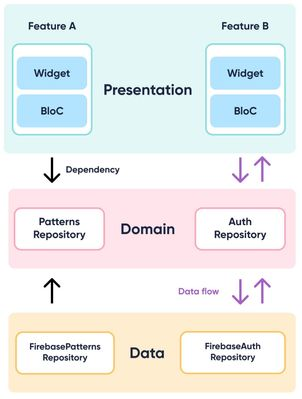
\includegraphics[width=0.5\textwidth]{images/firebase-architecture-BLoC.jpeg}
    \caption{Clean Architecture et BLoC pour la structure de l'application. (image récupérée sur \cite{googleCloudArchitecture})
    }
    \label{fig:architecture}
\end{figure}


%Des mainteneurs spécialisés testent les produits et certifient les informations, assurant ainsi la fiabilité des données fournies